
%(BEGIN_QUESTION)
% Copyright 2010, Tony R. Kuphaldt, released under the Creative Commons Attribution License (v 1.0)
% This means you may do almost anything with this work of mine, so long as you give me proper credit

To endebrytere skal tilkobles h.h.v. \texttt{Ix.5} og \texttt{Ix.11} på en Siemens SM-321 DI inngangsmodul.(model 6ES7321-1BL00-0AA0) Tegn de nødvendige koblingene. Det internekoblingsskjemaet for (\texttt{Ix.0}) vises som en referanse for alle inngangene.
Tegn de nødvendige koblingene som er nødvendig for tilkobling av endebryterene.  


$$\includegraphics[width=15.5cm]{i02508x01.eps}$$

Er dette en \textit{sinking} eller en \textit{sourcing} DI modul?
Tegn strømretning på alle ledere til IO-modulen. 
\vfil 

\underbar{file i02508}
\eject
%(END_QUESTION)





%(BEGIN_ANSWER)

This is an {\it input} PLC card, and so it receives electric current from a sensing device (e.g. a limit switch) to tell the PLC's microprocessor whether the sensor has been triggered or not.  Looking at the input card's internal circuitry, we see an optocoupler (LED and phototransistor) used to connect the interface circuitry with the real-world sensor signal.  In order to turn this phototransistor on, the LED must become forward-biased.

In order for the photocoupler's LED to become forward-biased, we must have direct current flowing downward through it (conventional flow notation).  This tells us the necessary direction of sensor current into the card: current enters in the L+ terminal, exiting the respective I/O channel terminal.  Since the L+ terminal is the ``common'' terminal for all 16 inputs on this particular card, it must be connected to the positive pole of a DC power supply.  Each limit switch must then be connected to the DC supply's negative pole, sinking current from the respective channels of the input card:

$$\includegraphics[width=15.5cm]{i02508x02.eps}$$

This particular input card is the {\it sourcing} type (arrows drawn in the direction of conventional flow).

%(END_ANSWER)





%(BEGIN_NOTES)


%INDEX% PLC, I/O: discrete I/O device wiring

%(END_NOTES)


